\documentclass[twoside]{book}

% Packages required by doxygen
\usepackage{fixltx2e}
\usepackage{calc}
\usepackage{doxygen}
\usepackage[export]{adjustbox} % also loads graphicx
\usepackage{graphicx}
\usepackage[utf8]{inputenc}
\usepackage{makeidx}
\usepackage{multicol}
\usepackage{multirow}
\PassOptionsToPackage{warn}{textcomp}
\usepackage{textcomp}
\usepackage[nointegrals]{wasysym}
\usepackage[table]{xcolor}

% Font selection
\usepackage[T1]{fontenc}
\usepackage[scaled=.90]{helvet}
\usepackage{courier}
\usepackage{amssymb}
\usepackage{sectsty}
\renewcommand{\familydefault}{\sfdefault}
\allsectionsfont{%
  \fontseries{bc}\selectfont%
  \color{darkgray}%
}
\renewcommand{\DoxyLabelFont}{%
  \fontseries{bc}\selectfont%
  \color{darkgray}%
}
\newcommand{\+}{\discretionary{\mbox{\scriptsize$\hookleftarrow$}}{}{}}

% Page & text layout
\usepackage{geometry}
\geometry{%
  a4paper,%
  top=2.5cm,%
  bottom=2.5cm,%
  left=2.5cm,%
  right=2.5cm%
}
\tolerance=750
\hfuzz=15pt
\hbadness=750
\setlength{\emergencystretch}{15pt}
\setlength{\parindent}{0cm}
\setlength{\parskip}{3ex plus 2ex minus 2ex}
\makeatletter
\renewcommand{\paragraph}{%
  \@startsection{paragraph}{4}{0ex}{-1.0ex}{1.0ex}{%
    \normalfont\normalsize\bfseries\SS@parafont%
  }%
}
\renewcommand{\subparagraph}{%
  \@startsection{subparagraph}{5}{0ex}{-1.0ex}{1.0ex}{%
    \normalfont\normalsize\bfseries\SS@subparafont%
  }%
}
\makeatother

% Headers & footers
\usepackage{fancyhdr}
\pagestyle{fancyplain}
\fancyhead[LE]{\fancyplain{}{\bfseries\thepage}}
\fancyhead[CE]{\fancyplain{}{}}
\fancyhead[RE]{\fancyplain{}{\bfseries\leftmark}}
\fancyhead[LO]{\fancyplain{}{\bfseries\rightmark}}
\fancyhead[CO]{\fancyplain{}{}}
\fancyhead[RO]{\fancyplain{}{\bfseries\thepage}}
\fancyfoot[LE]{\fancyplain{}{}}
\fancyfoot[CE]{\fancyplain{}{}}
\fancyfoot[RE]{\fancyplain{}{\bfseries\scriptsize Generated by Doxygen }}
\fancyfoot[LO]{\fancyplain{}{\bfseries\scriptsize Generated by Doxygen }}
\fancyfoot[CO]{\fancyplain{}{}}
\fancyfoot[RO]{\fancyplain{}{}}
\renewcommand{\footrulewidth}{0.4pt}
\renewcommand{\chaptermark}[1]{%
  \markboth{#1}{}%
}
\renewcommand{\sectionmark}[1]{%
  \markright{\thesection\ #1}%
}

% Indices & bibliography
\usepackage{natbib}
\usepackage[titles]{tocloft}
\setcounter{tocdepth}{3}
\setcounter{secnumdepth}{5}
\makeindex

% Hyperlinks (required, but should be loaded last)
\usepackage{ifpdf}
\ifpdf
  \usepackage[pdftex,pagebackref=true]{hyperref}
\else
  \usepackage[ps2pdf,pagebackref=true]{hyperref}
\fi
\hypersetup{%
  colorlinks=true,%
  linkcolor=blue,%
  citecolor=blue,%
  unicode%
}

% Custom commands
\newcommand{\clearemptydoublepage}{%
  \newpage{\pagestyle{empty}\cleardoublepage}%
}

\usepackage{caption}
\captionsetup{labelsep=space,justification=centering,font={bf},singlelinecheck=off,skip=4pt,position=top}

%===== C O N T E N T S =====

\begin{document}

% Titlepage & ToC
\hypersetup{pageanchor=false,
             bookmarksnumbered=true,
             pdfencoding=unicode
            }
\pagenumbering{roman}
\begin{titlepage}
\vspace*{7cm}
\begin{center}%
{\Large My Project }\\
\vspace*{1cm}
{\large Generated by Doxygen 1.8.11}\\
\end{center}
\end{titlepage}
\clearemptydoublepage
\tableofcontents
\clearemptydoublepage
\pagenumbering{arabic}
\hypersetup{pageanchor=true}

%--- Begin generated contents ---
\chapter{File Index}
\section{File List}
Here is a list of all files with brief descriptions\+:\begin{DoxyCompactList}
\item\contentsline{section}{\hyperlink{Lab1_8c}{Lab1.\+c} }{\pageref{Lab1_8c}}{}
\end{DoxyCompactList}

\chapter{File Documentation}
\hypertarget{FibonacciMatrix_8cpp}{}\section{Fibonacci\+Matrix.\+cpp File Reference}
\label{FibonacciMatrix_8cpp}\index{Fibonacci\+Matrix.\+cpp@{Fibonacci\+Matrix.\+cpp}}
{\ttfamily \#include $<$cstring$>$}\\*
{\ttfamily \#include $<$iostream$>$}\\*
{\ttfamily \#include $<$cstdlib$>$}\\*
Include dependency graph for Fibonacci\+Matrix.\+cpp\+:
\nopagebreak
\begin{figure}[H]
\begin{center}
\leavevmode
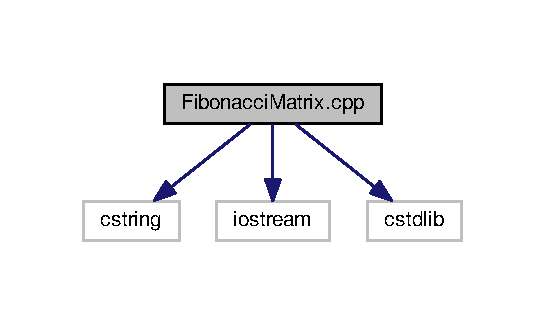
\includegraphics[width=262pt]{FibonacciMatrix_8cpp__incl}
\end{center}
\end{figure}
\subsection*{Macros}
\begin{DoxyCompactItemize}
\item 
\#define \hyperlink{FibonacciMatrix_8cpp_ae1d1ec9482079231e898236e2b23c9ba}{ll}~long long
\end{DoxyCompactItemize}
\subsection*{Functions}
\begin{DoxyCompactItemize}
\item 
void \hyperlink{FibonacciMatrix_8cpp_a2ced2a14bffe0cd7f9f38fea12982541}{multiply} (\hyperlink{FibonacciMatrix_8cpp_ae1d1ec9482079231e898236e2b23c9ba}{ll} F\mbox{[}2\mbox{]}\mbox{[}2\mbox{]}, \hyperlink{FibonacciMatrix_8cpp_ae1d1ec9482079231e898236e2b23c9ba}{ll} M\mbox{[}2\mbox{]}\mbox{[}2\mbox{]})
\item 
void \hyperlink{FibonacciMatrix_8cpp_a40ff419e8bf46e84041cdb03766f13d6}{power} (\hyperlink{FibonacciMatrix_8cpp_ae1d1ec9482079231e898236e2b23c9ba}{ll} F\mbox{[}2\mbox{]}\mbox{[}2\mbox{]}, int n)
\item 
\hyperlink{FibonacciMatrix_8cpp_ae1d1ec9482079231e898236e2b23c9ba}{ll} \hyperlink{FibonacciMatrix_8cpp_a048d1089c79b4503094e338aca490993}{fibo\+\_\+matrix} (\hyperlink{FibonacciMatrix_8cpp_ae1d1ec9482079231e898236e2b23c9ba}{ll} n)
\item 
int \hyperlink{FibonacciMatrix_8cpp_ae66f6b31b5ad750f1fe042a706a4e3d4}{main} ()
\end{DoxyCompactItemize}


\subsection{Macro Definition Documentation}
\index{Fibonacci\+Matrix.\+cpp@{Fibonacci\+Matrix.\+cpp}!ll@{ll}}
\index{ll@{ll}!Fibonacci\+Matrix.\+cpp@{Fibonacci\+Matrix.\+cpp}}
\subsubsection[{\texorpdfstring{ll}{ll}}]{\setlength{\rightskip}{0pt plus 5cm}\#define ll~long long}\hypertarget{FibonacciMatrix_8cpp_ae1d1ec9482079231e898236e2b23c9ba}{}\label{FibonacciMatrix_8cpp_ae1d1ec9482079231e898236e2b23c9ba}


\subsection{Function Documentation}
\index{Fibonacci\+Matrix.\+cpp@{Fibonacci\+Matrix.\+cpp}!fibo\+\_\+matrix@{fibo\+\_\+matrix}}
\index{fibo\+\_\+matrix@{fibo\+\_\+matrix}!Fibonacci\+Matrix.\+cpp@{Fibonacci\+Matrix.\+cpp}}
\subsubsection[{\texorpdfstring{fibo\+\_\+matrix(ll n)}{fibo_matrix(ll n)}}]{\setlength{\rightskip}{0pt plus 5cm}{\bf ll} fibo\+\_\+matrix (
\begin{DoxyParamCaption}
\item[{{\bf ll}}]{n}
\end{DoxyParamCaption}
)}\hypertarget{FibonacciMatrix_8cpp_a048d1089c79b4503094e338aca490993}{}\label{FibonacciMatrix_8cpp_a048d1089c79b4503094e338aca490993}

\begin{DoxyCode}
43 \{
44     \hyperlink{FibonacciMatrix_8cpp_ae1d1ec9482079231e898236e2b23c9ba}{ll} F[2][2] = \{\{1,1\},\{1,0\}\};
45     \textcolor{keywordflow}{if} (n == 0)
46         \textcolor{keywordflow}{return} 0;
47     \hyperlink{FibonacciMatrix_8cpp_a40ff419e8bf46e84041cdb03766f13d6}{power}(F, n - 1);
48     \textcolor{keywordflow}{return} F[0][0];
49 \}
\end{DoxyCode}


Here is the call graph for this function\+:
\nopagebreak
\begin{figure}[H]
\begin{center}
\leavevmode
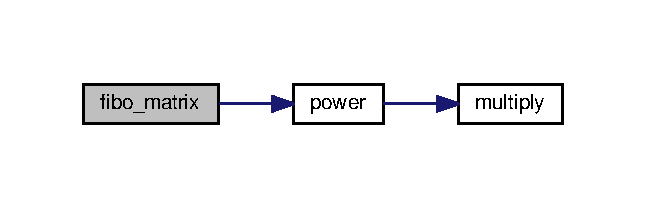
\includegraphics[width=310pt]{FibonacciMatrix_8cpp_a048d1089c79b4503094e338aca490993_cgraph}
\end{center}
\end{figure}


\index{Fibonacci\+Matrix.\+cpp@{Fibonacci\+Matrix.\+cpp}!main@{main}}
\index{main@{main}!Fibonacci\+Matrix.\+cpp@{Fibonacci\+Matrix.\+cpp}}
\subsubsection[{\texorpdfstring{main()}{main()}}]{\setlength{\rightskip}{0pt plus 5cm}int main (
\begin{DoxyParamCaption}
{}
\end{DoxyParamCaption}
)}\hypertarget{FibonacciMatrix_8cpp_ae66f6b31b5ad750f1fe042a706a4e3d4}{}\label{FibonacciMatrix_8cpp_ae66f6b31b5ad750f1fe042a706a4e3d4}

\begin{DoxyCode}
54 \{
55     \textcolor{keywordtype}{int} n;
56     \textcolor{keywordflow}{while} (1)
57     \{
58         cout<<\textcolor{stringliteral}{"Enter the integer n to find nth fibonnaci no.(0 to exit): "};
59         cin>>n;
60         \textcolor{keywordflow}{if} (n == 0)
61             \textcolor{keywordflow}{break};
62         cout<<\hyperlink{FibonacciMatrix_8cpp_a048d1089c79b4503094e338aca490993}{fibo\_matrix}(n)<<endl;
63     \}
64     \textcolor{keywordflow}{return} 0;
65 \}\end{DoxyCode}


Here is the call graph for this function\+:
\nopagebreak
\begin{figure}[H]
\begin{center}
\leavevmode
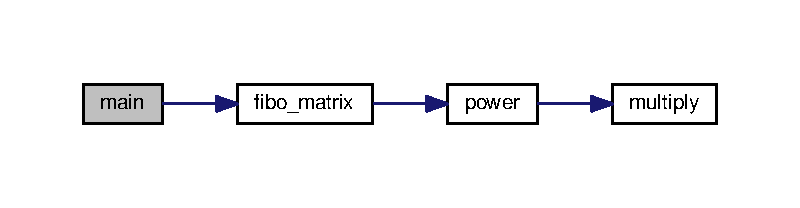
\includegraphics[width=350pt]{FibonacciMatrix_8cpp_ae66f6b31b5ad750f1fe042a706a4e3d4_cgraph}
\end{center}
\end{figure}


\index{Fibonacci\+Matrix.\+cpp@{Fibonacci\+Matrix.\+cpp}!multiply@{multiply}}
\index{multiply@{multiply}!Fibonacci\+Matrix.\+cpp@{Fibonacci\+Matrix.\+cpp}}
\subsubsection[{\texorpdfstring{multiply(ll F[2][2], ll M[2][2])}{multiply(ll F[2][2], ll M[2][2])}}]{\setlength{\rightskip}{0pt plus 5cm}void multiply (
\begin{DoxyParamCaption}
\item[{{\bf ll}}]{F\mbox{[}2\mbox{]}\mbox{[}2\mbox{]}, }
\item[{{\bf ll}}]{M\mbox{[}2\mbox{]}\mbox{[}2\mbox{]}}
\end{DoxyParamCaption}
)}\hypertarget{FibonacciMatrix_8cpp_a2ced2a14bffe0cd7f9f38fea12982541}{}\label{FibonacciMatrix_8cpp_a2ced2a14bffe0cd7f9f38fea12982541}

\begin{DoxyCode}
14 \{
15     \hyperlink{FibonacciMatrix_8cpp_ae1d1ec9482079231e898236e2b23c9ba}{ll} x =  F[0][0] * M[0][0] + F[0][1] * M[1][0];
16     \hyperlink{FibonacciMatrix_8cpp_ae1d1ec9482079231e898236e2b23c9ba}{ll} y =  F[0][0] * M[0][1] + F[0][1] * M[1][1];
17     \hyperlink{FibonacciMatrix_8cpp_ae1d1ec9482079231e898236e2b23c9ba}{ll} z =  F[1][0] * M[0][0] + F[1][1] * M[1][0];
18     \hyperlink{FibonacciMatrix_8cpp_ae1d1ec9482079231e898236e2b23c9ba}{ll} w =  F[1][0] * M[0][1] + F[1][1] * M[1][1];
19     F[0][0] = x;
20     F[0][1] = y;
21     F[1][0] = z;
22     F[1][1] = w;
23 \}
\end{DoxyCode}
\index{Fibonacci\+Matrix.\+cpp@{Fibonacci\+Matrix.\+cpp}!power@{power}}
\index{power@{power}!Fibonacci\+Matrix.\+cpp@{Fibonacci\+Matrix.\+cpp}}
\subsubsection[{\texorpdfstring{power(ll F[2][2], int n)}{power(ll F[2][2], int n)}}]{\setlength{\rightskip}{0pt plus 5cm}void power (
\begin{DoxyParamCaption}
\item[{{\bf ll}}]{F\mbox{[}2\mbox{]}\mbox{[}2\mbox{]}, }
\item[{int}]{n}
\end{DoxyParamCaption}
)}\hypertarget{FibonacciMatrix_8cpp_a40ff419e8bf46e84041cdb03766f13d6}{}\label{FibonacciMatrix_8cpp_a40ff419e8bf46e84041cdb03766f13d6}

\begin{DoxyCode}
29 \{
30     \textcolor{keywordflow}{if} (n == 0 || n == 1)
31         \textcolor{keywordflow}{return};
32     \hyperlink{FibonacciMatrix_8cpp_ae1d1ec9482079231e898236e2b23c9ba}{ll} M[2][2] = \{\{1,1\},\{1,0\}\};
33     \hyperlink{FibonacciMatrix_8cpp_a40ff419e8bf46e84041cdb03766f13d6}{power}(F, n / 2);
34     \hyperlink{FibonacciMatrix_8cpp_a2ced2a14bffe0cd7f9f38fea12982541}{multiply}(F, F);
35     \textcolor{keywordflow}{if} (n % 2 != 0)
36         \hyperlink{FibonacciMatrix_8cpp_a2ced2a14bffe0cd7f9f38fea12982541}{multiply}(F, M);
37 \}
\end{DoxyCode}


Here is the call graph for this function\+:
\nopagebreak
\begin{figure}[H]
\begin{center}
\leavevmode
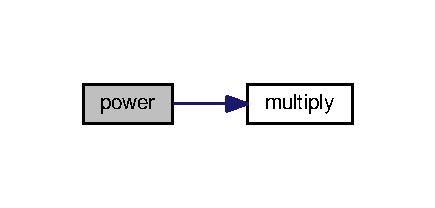
\includegraphics[width=209pt]{FibonacciMatrix_8cpp_a40ff419e8bf46e84041cdb03766f13d6_cgraph}
\end{center}
\end{figure}



%--- End generated contents ---

% Index
\backmatter
\newpage
\phantomsection
\clearemptydoublepage
\addcontentsline{toc}{chapter}{Index}
\printindex

\end{document}
